\documentclass[aspectratio=169,12pt]{beamer}

\usepackage{fontspec}
\setsansfont{Segoe UI}
\setmonofont{Consolas}
\newfontfamily\institutionfont{Times New Roman}
\usepackage{graphicx}
\usepackage{booktabs}
\usepackage{tabularx}
\usepackage{array}
\usepackage{colortbl}
\usepackage{ragged2e}
\usepackage{tikz}
\usetikzlibrary{arrows.meta,positioning,calc,fit,backgrounds,shapes.geometric}

\definecolor{Navy}{HTML}{14364A}
\definecolor{Teal}{HTML}{087E83}
\definecolor{Coral}{HTML}{D45C4B}
\definecolor{Amber}{HTML}{D6A72C}
\definecolor{Green}{HTML}{25865A}
\definecolor{Ink}{HTML}{1F2933}
\definecolor{Steel}{HTML}{71808A}
\definecolor{Ice}{HTML}{EAF5F6}
\definecolor{WarmGray}{HTML}{F2F1EE}
\definecolor{SoftWhite}{HTML}{FAFBFB}
\definecolor{Rule}{HTML}{D2DADD}
\definecolor{tcAccent}{RGB}{44,97,100}
\definecolor{tcGraphite}{RGB}{42,42,42}
\definecolor{tcSurface}{RGB}{250,250,250}

\setbeamercolor{normal text}{fg=Ink,bg=white}
\setbeamercolor{frametitle}{fg=Navy,bg=white}
\setbeamercolor{footline}{fg=Steel,bg=SoftWhite}
\setbeamerfont{frametitle}{size=\Large,series=\bfseries}
\setbeamertemplate{navigation symbols}{}
\setbeamersize{text margin left=0.68cm,text margin right=0.68cm}

\setbeamertemplate{frametitle}{%
  \nointerlineskip
  \begin{beamercolorbox}[wd=\paperwidth,ht=0.78cm,dp=0.18cm,leftskip=0.70cm,rightskip=1.45cm]{frametitle}
    \usebeamerfont{frametitle}\insertframetitle
  \end{beamercolorbox}
  \begin{tikzpicture}[remember picture,overlay]
    \fill[Teal] ([yshift=-0.01cm]current page.north west) ++(0,-0.96cm)
      rectangle ++(\paperwidth,0.035cm);
    \node[anchor=north east,inner sep=0pt] at
      ([xshift=-0.42cm,yshift=-0.13cm]current page.north east)
      {
\includegraphics[height=0.62cm]{assets/ATM.png}};
  \end{tikzpicture}%
}

\setbeamertemplate{footline}{%
  \begin{tikzpicture}[remember picture,overlay]
    \node[anchor=south east,inner sep=0pt,font=\scriptsize,text=Steel] at
      ([xshift=-0.40cm,yshift=0.22cm]current page.south east)
      {\insertframenumber};
  \end{tikzpicture}%
}

\newcommand{\statusdot}[1]{%
  \tikz[baseline=-0.55ex]\fill[#1] (0,0) circle (0.085cm);%
}

\newcommand{\objectivebox}[2]{%
  \tikz[baseline=(objective.center)]{%
    \node[
      draw=tcAccent,
      rounded corners=4pt,
      line width=0.72pt,
      fill=tcSurface,
      text=tcGraphite,
      minimum height=2.40cm,
      inner xsep=0.17cm,
      inner ysep=0.12cm
    ] (objective) {%
      \parbox[c][2.05cm][c]{5.18cm}{%
        \centering
        \offinterlineskip
        \parbox[c][0.48cm][c]{5.08cm}{%
          \centering\fontsize{10}{11.4}\selectfont\bfseries #1%
        }\par
        \vspace{0.08cm}
        \parbox[c][1.28cm][c]{5.08cm}{%
          \centering\fontsize{8.8}{10.2}\selectfont #2%
        }\par
      }%
    };
  }%
}

\newcommand{\validationrow}[2]{%
  \parbox[c][0.88cm][c]{3.15cm}{\centering\bfseries #1} &
  \parbox[c][0.88cm][c]{10.50cm}{\raggedright #2} \\
  \hline
}

\begin{document}

% Timing target: 0:20
% -----------------------------------------------------------------------------
% 1. Cover - composition matched to the supplied institutional example.
% -----------------------------------------------------------------------------
\begin{frame}[plain]
\begin{tikzpicture}[remember picture,overlay]
  \fill[white] (current page.south west) rectangle (current page.north east);

  \node[anchor=north,align=center,text width=15.20cm,
    font=\institutionfont\fontsize{9.3}{10.8}\selectfont\bfseries,text=Navy] at
    ([yshift=-0.25cm]current page.north)
    {ROMÂNIA\\
     MINISTERUL APĂRĂRII NAȚIONALE\\
     ACADEMIA TEHNICĂ MILITARĂ „FERDINAND I”\\
     FACULTATEA DE SISTEME INFORMATICE ȘI SECURITATE CIBERNETICĂ};

  \node[anchor=north,inner sep=0pt] at
    ([yshift=-1.95cm]current page.north)
    {
\includegraphics[height=1.35cm]{assets/ATM.png}};

  \node[anchor=center,align=center,text width=14.60cm,
    font=\fontsize{18}{22}\selectfont\bfseries,text=black] at
    ([yshift=0.25cm]current page.center)
    {\mbox{Soluție securizată de acces distant la resurse}\\
     cu autentificare multifactor};

  \node[anchor=north west,align=left,text width=6.70cm,
    font=\fontsize{8.6}{10.0}\selectfont,text=black] at
    ([xshift=1.35cm,yshift=-6.10cm]current page.north west)
    {\textbf{Conducător științific}\\[-0.02cm]
     Lect. Univ. Dr. Ing. Alin-Marian PUNCIOIU};

  \node[anchor=north east,align=right,text width=6.00cm,
    font=\fontsize{8.6}{10.0}\selectfont,text=black] at
    ([xshift=-1.35cm,yshift=-6.10cm]current page.north east)
    {\textbf{Absolvent}\\[-0.02cm]
     Sd. Sg. Maj. Maria-Laura ȘANDRU};

  \node[anchor=south,align=center,font=\fontsize{8.6}{10.0}\selectfont\bfseries,text=black] at
    ([yshift=0.45cm]current page.south)
    {București\\2026};
\end{tikzpicture}
\end{frame}

% Timing target: 0:20
% -----------------------------------------------------------------------------
% 2. Contents
% -----------------------------------------------------------------------------
\begin{frame}{Cuprins}
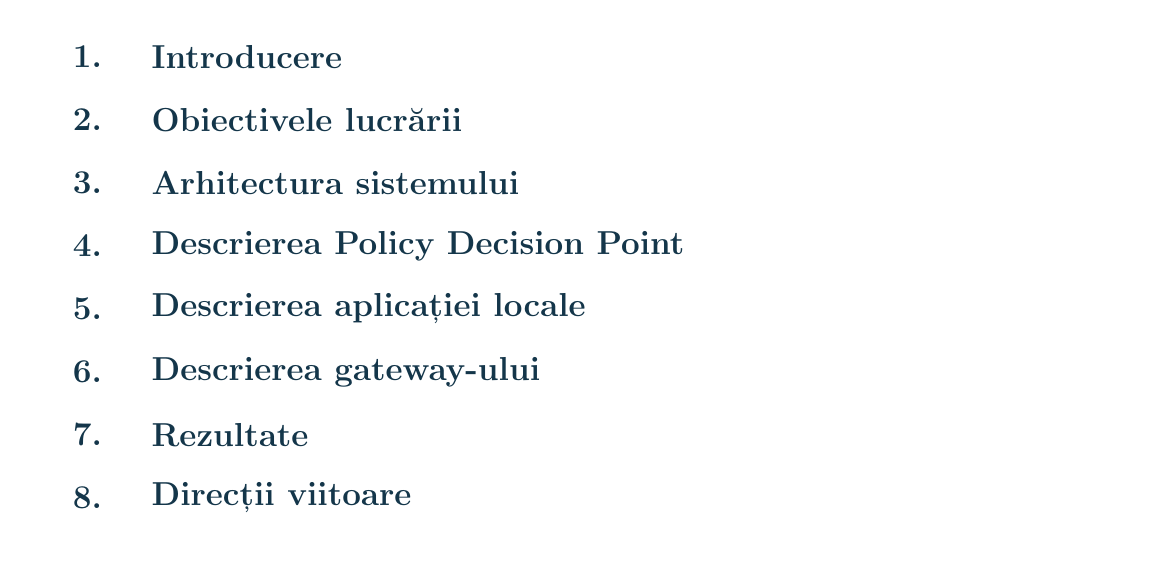
\begin{tikzpicture}[
  num/.style={anchor=east,inner sep=0pt,text=Navy,font=\large\bfseries},
  entry/.style={anchor=west,align=left,text width=11.55cm,font=\large\bfseries,text=Navy}
]
  \path[use as bounding box] (0,0) rectangle (14,6.55);

  \node[num] at (0.95,6.18) {1.};
  \node[entry] at (1.45,6.18) {Introducere};

  \node[num] at (0.95,5.38) {2.};
  \node[entry] at (1.45,5.38) {Obiectivele lucrării};

  \node[num] at (0.95,4.58) {3.};
  \node[entry] at (1.45,4.58) {Arhitectura sistemului};

  \node[num] at (0.95,3.78) {4.};
  \node[entry] at (1.45,3.78) {Descrierea Policy Decision Point};

  \node[num] at (0.95,2.98) {5.};
  \node[entry] at (1.45,2.98) {Descrierea aplicației locale};

  \node[num] at (0.95,2.18) {6.};
  \node[entry] at (1.45,2.18) {Descrierea gateway-ului};

  \node[num] at (0.95,1.38) {7.};
  \node[entry] at (1.45,1.38) {Rezultate};

  \node[num] at (0.95,0.58) {8.};
  \node[entry] at (1.45,0.58) {Direcții viitoare};
\end{tikzpicture}
\end{frame}

% Timing target: 0:40
% -----------------------------------------------------------------------------
% 3. Introduction
% -----------------------------------------------------------------------------
\begin{frame}{Introducere}
\vfill
{%
\setbeamercolor{itemize item}{fg=Teal}
\setbeamertemplate{itemize item}{\raisebox{0.12ex}{\scriptsize$\bullet$}}
\small
\begin{itemize}
  \setlength{\itemsep}{0.23cm}
  \item \textbf{Acces distant la resurse}
  \item \textbf{Limitele modelului de securitate perimetrală}
  \item \textbf{Zero-Trust}
\end{itemize}
}
\vfill
\end{frame}

% Timing target: 0:50
% -----------------------------------------------------------------------------
% 4. Relevance and objectives
% -----------------------------------------------------------------------------
\begin{frame}{Obiectivele lucrării}
\vspace{0.10cm}
\begingroup
\noindent\makebox[\linewidth][c]{%
  \objectivebox{Evaluare continuă a accesului}{Verificarea identității, dispozitivului și contextului la inițierea accesului și pe durata sesiunii.}%
  \hspace{0.24cm}%
  \objectivebox{Control granular al accesului}{Aplicarea principiului privilegiului minim, fără expunerea întregii rețele interne.}%
}

\vspace{0.30cm}
\noindent\makebox[\linewidth][c]{%
  \objectivebox{Control contextual al accesului}{Acordarea sau refuzarea accesului și solicitarea MFA în funcție de context.}%
}
\endgroup
\end{frame}

% Timing target: 1:00
% -----------------------------------------------------------------------------
% 5. Architecture
% -----------------------------------------------------------------------------
\begin{frame}{Arhitectura sistemului}
\begin{tikzpicture}[remember picture,overlay]
  \node[inner sep=0pt] at ([xshift=-0.65cm,yshift=-0.65cm]current page.center) {%
    \resizebox{0.92\textwidth}{!}{% Exact diagram from thesis_doc/components/images/diagrams/implementation_architecture.tex.
% Only the icon paths are adjusted for the self-contained presentation folder.
\definecolor{tcCoolSteel}{RGB}{160,166,168}
\definecolor{tcAccent}{RGB}{44,97,100}
\definecolor{tcGraphite}{RGB}{42,42,42}
\definecolor{tcSurface}{RGB}{250,250,250}
\definecolor{tcSurfaceCard}{RGB}{238,238,236}
\definecolor{tcBorder}{RGB}{196,200,200}
\begingroup
\renewcommand{\tiny}{\fontsize{5}{6}\selectfont}
\renewcommand{\scriptsize}{\fontsize{7}{8}\selectfont}
\renewcommand{\footnotesize}{\fontsize{8}{10}\selectfont}
\renewcommand{\small}{\fontsize{9}{11}\selectfont}
\renewcommand{\normalsize}{\fontsize{10}{12}\selectfont}
\renewcommand{\large}{\fontsize{12}{14}\selectfont}
\renewcommand{\Large}{\fontsize{14.4}{18}\selectfont}
\normalsize
\begin{tikzpicture}[
    pdpcontainer/.style={draw=tcAccent, rounded corners=5pt, line width=0.85pt, fill=tcSurface, minimum width=5.70cm, minimum height=3.88cm},
    pdpinner/.style={draw=tcAccent, rounded corners=4pt, align=center, text width=4.30cm, minimum width=4.70cm, minimum height=0.82cm, fill=tcSurface, text=tcGraphite, line width=0.72pt},
    support/.style={draw=tcAccent, rounded corners=4pt, align=center, text width=2.05cm, minimum width=2.40cm, minimum height=1.55cm, fill=tcSurface, text=tcGraphite, line width=0.72pt},
    data/.style={draw=tcAccent, rounded corners=4pt, align=center, text width=1.45cm, minimum width=1.80cm, minimum height=1.95cm, fill=tcSurface, text=tcGraphite, line width=0.72pt},
    pep/.style={draw=tcAccent, rounded corners=4pt, align=center, text width=2.55cm, minimum width=3.00cm, minimum height=1.95cm, fill=tcSurface, text=tcGraphite, line width=0.72pt},
    arrow/.style={-{Stealth[length=2.2mm]}, line width=0.78pt, draw=tcAccent},
    dataarrow/.style={-{Stealth[length=2.4mm]}, line width=0.95pt, draw=tcAccent},
    controlbi/.style={<->, >=Stealth, line width=0.78pt, draw=tcAccent},
    internalbi/.style={<->, >=Stealth, line width=0.60pt, draw=tcAccent, shorten <=1pt, shorten >=1pt},
    label/.style={font=\small, text=tcGraphite}
]

\path[use as bounding box] (0.00,0.25) rectangle (14.00,8.08);

% Plane separation
\draw[densely dashed, line width=0.75pt, draw=tcCoolSteel] (0.80,3.55) -- (13.20,3.55);
\node[anchor=west, label] at (0.95,3.88) {Planul de control};
\node[anchor=west, label] at (0.95,3.22) {Planul de date};

% Control plane
\node[support] (db) at (2.00,7.08) {
\includegraphics[height=0.90cm]{assets/postgres-icon.png}\\[0.03cm]PostgreSQL};
\node[support] (redis) at (2.00,5.34) {
\includegraphics[height=0.90cm]{assets/redis-icon.png}\\[0.03cm]Redis};

\node[pdpcontainer] (pdpbox) at (7.00,6.22) {};
\node[align=center] at (7.00,7.68) {%
    
\includegraphics[height=0.90cm]{assets/go-icon.png}\hspace{0.36cm}%
    
\includegraphics[height=0.90cm]{assets/react-icon.png}};
\node[pdpinner] (pe) at (7.00,6.62) {Policy Engine};
\node[pdpinner] (pa) at (7.00,5.34) {Policy Administrator};
\node[font=\normalsize,text=tcGraphite] at (7.00,4.58) {Policy Decision Point};

\node[support] (vault) at (12.00,7.18) {
\includegraphics[height=0.90cm]{assets/hashicorp-icon.png}\\[0.03cm]Vault};
\node[support] (idp) at (12.00,5.44) {Furnizori\\OIDC};

% Data plane
\node[align=center, inner sep=1pt] (user) at (1.45,1.55) {
\includegraphics[height=0.90cm]{assets/user-icon.png}};
\node[pep] (localapp) at (4.05,1.55) {
\includegraphics[height=0.90cm]{assets/wails-icon.png}\hspace{0.24cm}
\includegraphics[height=0.90cm]{assets/go-icon.png}\\Agent};
\node[pep] (gateway) at (8.65,1.55) {
\includegraphics[height=0.90cm]{assets/go-icon.png}\\Gateway};
\node[data] (resource) at (12.10,1.55) {Resurse};

% Control communication
\draw[arrow] (pdpbox.west |- db.east) -- (db.east);
\draw[arrow] (pdpbox.west |- redis.east) -- (redis.east);
\draw[arrow] (pdpbox.east |- vault.west) -- (vault.west);
\draw[arrow] (pdpbox.east |- idp.west) -- (idp.west);
\draw[internalbi, shorten <=0pt, shorten >=0pt] (pe.south) -- (pa.north);
\draw[controlbi, shorten <=0pt, shorten >=0pt] (localapp.north) -- (6.50,4.28);
\draw[controlbi, shorten <=0pt, shorten >=0pt] (gateway.north) -- (7.12,4.28);

% Data path
\draw[dataarrow] (user) -- (localapp);
\draw[dataarrow] (localapp) -- (gateway);
\draw[dataarrow] (gateway) -- (resource);

\end{tikzpicture}
\endgroup
}%
  };
\end{tikzpicture}
\end{frame}

% Timing target: 1:00
% -----------------------------------------------------------------------------
% 4. Identity and policy decision
% -----------------------------------------------------------------------------
\begin{frame}{Descrierea Policy Decision Point}
\vfill
{%
\setbeamercolor{itemize item}{fg=Teal}
\setbeamertemplate{itemize item}{\raisebox{0.12ex}{\scriptsize$\bullet$}}
\small
\begin{itemize}
  \setlength{\itemsep}{0.23cm}
  \item \textbf{Interfață de administrare:} configurare furnizori de identitate, gateway-uri, resurse și politici.
  \item \textbf{Federarea și sincronizarea identităților:} autentifică utilizatorii prin OIDC cu PKCE și sincronizează utilizatorii și grupurile prin SCIM.
  \item \textbf{Integrare cu HashiCorp Vault:} utilizează PKI pentru emiterea certificatelor mTLS și Transit pentru protejarea cheilor și secretelor persistente.
  \item \textbf{Gestionează token-urile de acces:} emite token-uri opace pentru sesiunile de acces la resurse și token-uri JWT pentru autentificarea în aplicația locală.
  \item \textbf{Evaluează politicile și stabilește decizia de acces:} corelează utilizatorul, grupurile, dispozitivul, politicile de acces și resursa solicitată, apoi acordă accesul, solicită autentificare multifactor suplimentară prin TOTP/WebAuthn (passkeys) sau refuză cererea.
\end{itemize}
}
\vfill
\end{frame}

% Timing target: 1:10
% -----------------------------------------------------------------------------
% 7. Local application
% -----------------------------------------------------------------------------
\begin{frame}{Descrierea aplicației locale (Agent)}
\vspace{0.12cm}
{%
\setbeamercolor{itemize item}{fg=Teal}
\setbeamertemplate{itemize item}{\raisebox{0.12ex}{\scriptsize$\bullet$}}
\small
\begin{itemize}
  \setlength{\itemsep}{0.23cm}
  \item \textbf{Înrolează dispozitivul și autentifică utilizatorul:} generează o cheie ECDSA P-256 neexportabilă în TPM/Microsoft Software Key Storage Provider. Obține certificatul mTLS și inițiază fluxul de autentificare prin OIDC.
  \item \textbf{Colectează date despre dispozitiv:} actualizările Windows, politicile de parolă și blocare, starea antivirusului și firewall-ul.
  \item \textbf{Controlează rezoluția numelor:} configurează NRPT, resolver-ul DNS local și asociază fiecărei resurse un IP sintetic din intervalul CGNAT.
  \item \textbf{Interceptează și autorizează traficul:} WFP redirecționează conexiunile către proxy-ul local, care identifică resursa și solicită decizia PDP.
  \item \textbf{Gestionează conexiunea securizată:} deschide tunelul TLS 1.3 mTLS cu Gateway-ul și multiplexează fluxurile prin yamux.
\end{itemize}
}
\end{frame}

% Timing target: 1:10
% -----------------------------------------------------------------------------
% 8. Gateway
% -----------------------------------------------------------------------------
\begin{frame}{Descrierea gateway-ului}
\vspace{0.12cm}
{%
\setbeamercolor{itemize item}{fg=Teal}
\setbeamertemplate{itemize item}{\raisebox{0.12ex}{\scriptsize$\bullet$}}
\small
\begin{itemize}
  \setlength{\itemsep}{0.23cm}
  \item \textbf{Izolarea resurselor interne:} gateway-ul acționează ca punct unic de acces către resursele protejate, asigurând rutarea controlată a traficului provenit de la aplicația locală.
  \item \textbf{Aplicarea deciziilor de acces:} pe baza deciziilor primite de la PDP, gateway-ul permite sau blochează accesul către resursele interne.
\end{itemize}
}
\end{frame}

% Timing target: 0:55
% -----------------------------------------------------------------------------
% 9. Functional validation
% -----------------------------------------------------------------------------
\begin{frame}[t]{Rezultate}
\vspace{0.16cm}
{\large\bfseries\color{Navy}Validarea scenariilor de acces}\par
\vspace{0.24cm}
{\fontsize{8.6}{9.8}\selectfont
\renewcommand{\arraystretch}{1}
\setlength{\arrayrulewidth}{0.45pt}
\arrayrulecolor{Rule}
\noindent\makebox[\linewidth][c]{%
\begin{tabular}{|c|c|}
  \hline
  \validationrow{Deplasare imposibilă}{Sesiunea anterioară este revocată, iar noul acces necesită verificare MFA.}
  \validationrow{Starea dispozitivului}{Accesul este menținut când dispozitivul este conform și revocat când o condiție relevantă nu mai este îndeplinită.}
  \validationrow{Modificări administrative}{Revocarea sesiunii sau dezactivarea resursei ori a gateway-ului oprește accesul activ și blochează cererile noi.}
  \validationrow{Rețeaua sursă}{Politica permite, refuză sau condiționează accesul prin MFA în funcție de adresa IP.}
  \validationrow{Cereri modificate}{Cererile fără certificat mTLS, cu token invalid sau cu parametri de conexiune diferiți de cei autorizați sunt respinse.}
  \validationrow{PDP indisponibil}{Nu pot fi create sau reînnoite sesiuni, iar gateway-ul acceptă numai sesiunile primite anterior, până la expirare.}
\end{tabular}%
}}
\end{frame}

% Timing target: 0:50
% -----------------------------------------------------------------------------
% 10. Performance results
% -----------------------------------------------------------------------------
\begin{frame}{Rezultate}
\vspace{0.03cm}
{\large\bfseries\color{Navy}Performanță}\par
\vspace{0.10cm}
\makebox[\linewidth][c]{%
  \resizebox{0.64\linewidth}{!}{%
  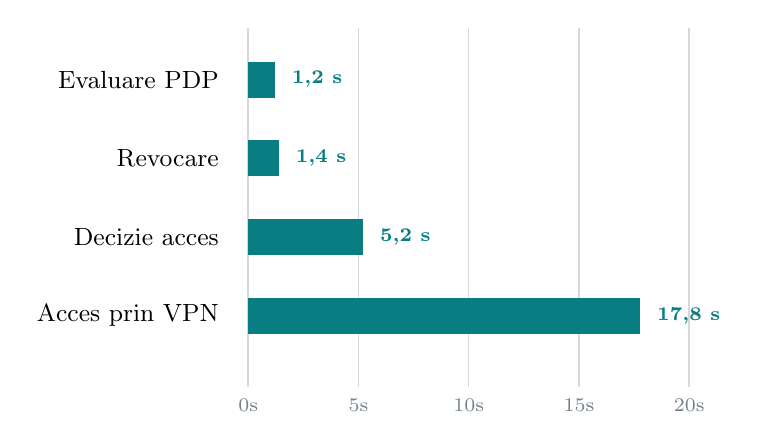
\begin{tikzpicture}[font=\small]
    \foreach \x/\label in {3.15/0,4.55/5,5.95/10,7.35/15,8.75/20}{
      \draw[Rule,line width=0.55pt] (\x,0.35) -- (\x,4.90);
      \node[font=\scriptsize,text=Steel] at (\x,0.12) {\label s};
    }
    \node[anchor=east] at (2.90,4.25) {Evaluare PDP};
    \fill[Teal] (3.15,4.02) rectangle ++(0.34,0.46);
    \node[anchor=west,font=\scriptsize\bfseries,text=Teal] at (3.58,4.25) {1,2 s};
    \node[anchor=east] at (2.90,3.25) {Revocare};
    \fill[Teal] (3.15,3.02) rectangle ++(0.39,0.46);
    \node[anchor=west,font=\scriptsize\bfseries,text=Teal] at (3.63,3.25) {1,4 s};
    \node[anchor=east] at (2.90,2.25) {Decizie acces};
    \fill[Teal] (3.15,2.02) rectangle ++(1.46,0.46);
    \node[anchor=west,font=\scriptsize\bfseries,text=Teal] at (4.70,2.25) {5,2 s};
    \node[anchor=east] at (2.90,1.25) {Acces prin VPN};
    \fill[Teal] (3.15,1.02) rectangle ++(4.98,0.46);
    \node[anchor=west,font=\scriptsize\bfseries,text=Teal] at (8.22,1.25) {17,8 s};
  \end{tikzpicture}%
  }%
}
\end{frame}

% Timing target: 0:45
% -----------------------------------------------------------------------------
% 11. Future work
% -----------------------------------------------------------------------------
\begin{frame}{Direcții viitoare}
\vspace{0.10cm}
\begingroup
\noindent\makebox[\linewidth][c]{%
  \objectivebox{Portabilitate}{Extinderea aplicației locale pentru Linux și macOS.}%
  \hspace{0.24cm}%
  \objectivebox{Extinderea MFA}{Adăugarea unor factori suplimentari, precum notificările push.}%
}

\vspace{0.30cm}
\noindent\makebox[\linewidth][c]{%
  \objectivebox{Risc adaptiv}{Integrarea unor modele de învățare automată pentru calcularea dinamică a scorului de risc.}%
}
\endgroup
\end{frame}

% Timing target: 0:25
% -----------------------------------------------------------------------------
% 12. Bibliography
% -----------------------------------------------------------------------------
\begin{frame}{Bibliografie}
\vspace{0.14cm}
{%
\setbeamertemplate{enumerate item}{\arabic{enumi}.}
\setbeamercolor{enumerate item}{fg=Navy}
\fontsize{8.7}{10.2}\selectfont
\begin{enumerate}
  \setlength{\itemsep}{0.15cm}
  \item S. Rose, O. Borchert, S. Mitchell și S. Connelly, \textit{Zero Trust Architecture}, NIST SP 800-207, 2020.
  \item M. Souppaya și K. Scarfone, \textit{Guide to Enterprise Telework, Remote Access, and BYOD Security}, NIST SP 800-46 Rev. 2, 2016.
  \item National Institute of Standards and Technology, \textit{Digital Identity Guidelines: Authentication and Lifecycle Management}, NIST SP 800-63B, 2025.
  \item OpenID Foundation, \textit{OpenID Connect Core 1.0 Incorporating Errata Set 2}, 2023.
  \item P. Hunt, K. Grizzle, M. Ansari, E. Wahlstroem și C. Mortimore, \textit{System for Cross-domain Identity Management: Protocol}, RFC 7644, 2015.
  \item World Wide Web Consortium, \textit{Web Authentication: An API for Accessing Public Key Credentials Level 3}, 2026.
  \item HashiCorp, \textit{Transit secrets engine}, 2026.
\end{enumerate}
}
\end{frame}

% Timing target: 0:10
% -----------------------------------------------------------------------------
% 13. Closing slide
% -----------------------------------------------------------------------------
\begin{frame}
\begin{tikzpicture}[remember picture,overlay]
  \fill[white] (current page.south west) rectangle (current page.north east);

  \node[anchor=north,align=center,text width=15.20cm,
    font=\institutionfont\fontsize{9.3}{10.8}\selectfont\bfseries,text=Navy] at
    ([yshift=-0.25cm]current page.north)
    {ROMÂNIA\\
     MINISTERUL APĂRĂRII NAȚIONALE\\
     ACADEMIA TEHNICĂ MILITARĂ „FERDINAND I”\\
     FACULTATEA DE SISTEME INFORMATICE ȘI SECURITATE CIBERNETICĂ};

  \node[anchor=north,inner sep=0pt] at
    ([yshift=-1.95cm]current page.north)
    {
\includegraphics[height=1.35cm]{assets/ATM.png}};

  \node[anchor=center,align=center,
    font=\fontsize{27}{32}\selectfont\bfseries,text=black] at
    ([yshift=-0.45cm]current page.center)
    {Vă mulțumesc pentru atenție!};

  \node[anchor=south west,align=left,text width=6.70cm,
    font=\fontsize{8.6}{10.0}\selectfont,text=black] at
    ([xshift=1.35cm,yshift=0.55cm]current page.south west)
    {\textbf{Conducător științific}\\[-0.02cm]
     Lect. Univ. Dr. Ing. Alin-Marian PUNCIOIU};

  \node[anchor=south east,align=right,text width=6.00cm,
    font=\fontsize{8.6}{10.0}\selectfont,text=black] at
    ([xshift=-1.35cm,yshift=0.55cm]current page.south east)
    {\textbf{Absolvent}\\[-0.02cm]
     Sd. Sg. Maj. Maria-Laura ȘANDRU};
\end{tikzpicture}
\end{frame}

\end{document}
